\documentclass[11pt,a4paper]{article}
\usepackage{graphicx}
\usepackage[utf8]{inputenc}
\usepackage[T1]{fontenc}
\usepackage{adjustbox}
\usepackage[english]{babel}
\usepackage{lmodern,microtype}
\usepackage[a4paper,margin=2cm,headheight=12pt]{geometry}
\usepackage{geometry}
\usepackage{graphicx}
\usepackage{amsmath,amssymb}
\usepackage{booktabs}
\usepackage{array}
\usepackage{tabularx}
\usepackage{adjustbox}
\usepackage{float}
\usepackage{caption}
\usepackage{setspace}

\geometry{margin=02cm}
\setlength{\parindent}{0pt}
\setlength{\parskip}{0.65em}
\renewcommand{\arraystretch}{1.2}


\usepackage{listings}
\usepackage{xcolor}


\lstdefinelanguage{json}{       
    basicstyle = \normalfont\ttfamily,
    stringstyle = \color{red!70!black}, 
    keyboardstyle = \color{blue},
    morestring = [b]", 
    tabsize = 4, 
    showstringspaces = false
}


\usepackage{setspace,parskip,enumitem,booktabs,longtable,xcolor,hyperref,fancyhdr,titlesec,listings}
\definecolor{bleu}{RGB}{26,65,110}
\definecolor{lien}{RGB}{20,75,140}
\hypersetup{colorlinks=true,linkcolor=bleu,urlcolor=lien,pdftitle={Our Report -- MALIS Project}}
\setstretch{1.1}
\setlist[itemize]{leftmargin=1.5em,itemsep=0.25em}
\setlist[enumerate]{leftmargin=1.7em,itemsep=0.35em}
\titleformat{\section}{\Large\bfseries\color{bleu}}{\thesection}{0.7em}{}
\titleformat{\subsection}{\large\bfseries\color{bleu}}{\thesubsection}{0.7em}{}
\pagestyle{fancy}\fancyhf{}\lhead{\small Our Report}\rhead{\small MALIS Project}\cfoot{\thepage}
\lstset{basicstyle=\ttfamily\small,breaklines=true,frame=single}
\begin{document}
\begin{titlepage}
\centering\vspace*{1.7cm}
{\Large\bfseries MALIS PROJECT REPORTING \par}
\vspace{1.2cm}
{\Huge\bfseries\color{bleu} MACHINE LEARNING AND INTELLIGENT SYSTEMS\par}
\vspace{0.5cm}
{\LARGE Reinforcement Learning and Multi-Armed Bandits\par}
\vspace{1.4cm}
\begin{tabular}{@{}ll@{}}
\textbf{Professor:} & A. Maria ZULUAGA \\

\textbf{Students :} & Sounsin Isaac Tychique DAKIO \\
                    &  Mengu PU \\
                    &  Shane Elton LEWIS \\
                
\end{tabular}

\vspace{2cm}

\begin{figure}[!h]
    \centering
    
\includegraphics[width=0.5\linewidth]{figures/image.png}
    \label{fig:placeholder}
\end{figure}

\vfill

\vspace{1cm}{\large \today\par}
\end{titlepage}


\section*{Introduction}

This project analyses an N-Armed Bandit problem i.e choices can be made from n options and each choice possesses a value that is based on a stationary probability action dependent on the action. The objective of this project is to maximise the value over a time step.
 
This project using a fishing.py simulator wherein the user/agent can choose between 5 fishing spots (Old Pier,Rocky Point, Seagrass Bed , Lighthouse Reef , Deep Channel) .The simulator is split across 3 seasons:
Season 1:A baseline season with 30 days
Season 2:A season that lasts only 10 days
Season 3:A season that is 30 days but non stationary and uses a different set of means after day 16 .
 
The following sections will analyse different methods and agents to maximise the output and compare it with the results from humans interacting with the simulator.



\section*{Task 2: Human strategies and outcomes}

\begin{itemize}
    \item \textbf{Pu Mengu:} In Season 1, Pu sampled all five spots, focused on Old Pier, and checked alternatives when catches fell, as described in her notes. She tried the same approach in the shorter Season 2 but, with limited observations, favored Rocky Point. In Season 3, she tested Lighthouse Reef and Rocky Point, switching after low catches at Lighthouse Reef. Her notes match this exploration-and-switching strategy, though she did not try Old Pier after the day-16 shift, when it became the best spot.

    \item \textbf{Dakio Isaac:} Dakio explored spots broadly and without a fixed order i.e randomly in Seasons 1 and 2. In Season 2 acccording to the log shows some repetition: Rocky Point was visited three times, while Deep Channel was visited once. In Season 3, he followed a more structured pattern, choosing nearby or recently visited spots. This matches his notes, including his decision to continue that pattern after the day-16 shift.

    \item \textbf{Shane Elton Lewis:} Lewis moved among spots to spread his choices in Season 1. In Season 2, after observing initial catches, he focused on Rocky Point and Lighthouse Reef. He began Season 3 by favoring Rocky Point, Seagrass Bed and Old Pier, then shifted toward Deep Channel after the change. His choices broadly match his notes; he first tried Deep Channel on day 22 and focused on it during the final six days.
\end{itemize}

\noindent\textbf{Human Rule derived from the team strategies:} Sample several or all spots, compare their observed catches, focus on those with the strongest results, and reassess alternatives when catches decline or conditions change. The ten-day Season 2 and the Season 3 shift limited how much evidence players could gather before adapting.


Our different results are summarized in this table : 
\begin{table}[H]\centering\large
\begin{tabular}{llrrr}\toprule
Player & Season 1 & Season 2 & Season 3 & Total (kg)\\\midrule
Pu Mengu & 236.8 & 74.4 & 185.6 & 496.8\\
Dakio Isaac & 155.2 & 75.0 & 167.5 & 397.7\\
Shane Lewis & 184.0 & 60.1 & 212.3 & 456.4\\\bottomrule
\end{tabular}
\caption{Observed catches by our team members.}
\end{table}







\section*{Task 3: Measuring decision performance}

This section proposes a performance measure to analyse intricately the results obtained from each team member . In order to realise this we propose a loss function defined by the following equation using mean  error .
\[
R_{\rm dec}=V^*-\sum_{t=1}^{T}\mu_{A_t,t},
\]
where $V^*$ is the expected catch, $A_t$ is the chosen spot, and $\mu_{A_t,t}$ is its true mean on day $t$. For Season 3, the calculation uses the means before and after day 16.
To distinguish decision quality from random reward variation, we define a luck residual as the difference between the realized and expected catches:

\[
L=\sum_{t=1}^{T}(R_t-\mu_{A_t,t})
\]

where \(R_t\) is the realized catch and \(\mu_{A_t,t}\) is the true expected catch of the selected spot on day \(t\).

The relationship between realized regret and decision regret can therefore be expressed as:

\[
R_{\mathrm{actual}}=R_{\mathrm{dec}}-L
\]

A positive luck residual indicates catches above expectations, while a negative residual indicates catches below expectations. Over repeated simulations, the mean residual should approach zero, assuming unbiased reward generation. This allows us to distinguish the quality of an agent's decisions from random fluctuations in its observed rewards.

\begin{table}[H]\centering\small
\begin{tabular}{lrrrr}\toprule
Player & Season 1 & Season 2 & Season 3 & Mean\\\midrule
Dakio & 121.3 & 22.9 & 104.2 & 82.8\\
Lewis & 72.5 & 10.7 & 49.6 & 44.3\\
Pu & 40.0 & 18.4 & 43.4 & 33.9\\\midrule
All players & & & & 53.7\\\bottomrule
\end{tabular}
\caption{Decision regret (kg) on each member's logged bays.}
\end{table}

To check that regret separates decisions from luck, we evaluated the same HumanRuleAgent on 1,000 random bays per season. Its mean realized and expected catches were close, but the luck residual varied across individual bays:

\begin{table}[H]\centering\small
\begin{tabular}{lrrrr}\toprule
Season & Mean expected catch & Mean realized catch & Mean decision regret & SD of luck residual\\\midrule
1 & 231.13 & 231.35 & 28.85 & 13.57\\
2 & 69.88 & 69.96 & 17.18 & 7.82\\
3 & 213.79 & 213.94 & 46.20 & 14.18\\\bottomrule
\end{tabular}
\caption{HumanRuleAgent results over 1,000 random bays per season (kg).}
\end{table}

The mean luck residuals were 0.23, 0.08 and 0.16 kg in Seasons 1--3, compared with residual standard deviations of 7.82--14.18 kg. Thus a single catch total can be noticeably affected by luck, while expected-catch regret evaluates the choices themselves.

Season 2 offered only ten choices, so its raw totals should be compared relative to each bay's oracle. The team members achieved 88.6\% (Pu), 81.5\% (Dakio) and 80.1\% (Lewis) of their Season 2 oracle totals, compared with 81.4\%, 57.5\% and 72.2\% in Season 1. 

Dakio sampled the new best spot quickly but continued rotating; Lewis adapted later and sustained his focus near the season's end. Pu changed spots after low catches but did not test the new best location.



\section*{Task 4: Bandit algorithms}
We compare three action-value algorithms with a rule-based human baseline. Each learns only from the catches it has observed and resets its estimates at the start of a season.
\subsection*{Greedy agent : }
Greedy chooses the spot with the highest current estimate:
\[
A_t=\arg\max_a Q_t(a).
\]
We test $Q_0=0$ and the optimistic value $Q_0=12$ kg. Optimistic estimates encourage early sampling of other spots.

\subsection*{Epsilon-greedy agent : }
With probability $\epsilon$, this agent chooses a spot uniformly at random; otherwise it chooses $\arg\max_a Q_t(a)$. The baseline uses $\epsilon=0.1$. Unlike optimistic initialization, epsilon-greedy continues random exploration throughout the season, which can also spend later choices on lower-value spots.

\subsection*{Upper Confidence Bound agent : }
UCB adds an uncertainty bonus to each estimated value:
\[
A_t=\arg\max_a\left[Q_t(a)+c\sqrt{\frac{\ln t}{N_t(a)}}\right].
\]
Here $N_t(a)$ counts visits to spot $a$, and $c$ controls exploration. We use $c=2$; untried spots are selected once before applying the score. The bonus then favors spots with fewer observations, unlike uniform random exploration.

\subsection*{Best human strategy and value updates : }
Pu had the highest aggregate human catch (496.8 kg), so her explore-then-exploit approach is the best overall human strategy in our Part II, although the remaining players led individual seasons. The  HumanRuleAgent in \texttt{agents.py} formalizes this approach: it samples every spot once, estimates each from up to its last three catches, and exploits the best estimate. If the mean of the last two catches at its current spot falls below a predefined threshold of 3 kg, it begins exploring for  the best estimated alternative. 

This is a repeatable approximation of Pu's strategy, not a replay of her exact choices. After each catch $R$, values update as $Q(a)\leftarrow Q(a)+\alpha(R-Q(a))$. Sample averages use $\alpha=1/N(a)$; constant $\alpha$ weights recent catches more and can track change.



\newpage

\section*{Task 5: Experiments and discussion}
\subsection*{Experimental protocol and random-bay results}
Our \texttt{experiment-2-contextual.ipynb} notebook imports every policy from \texttt{agents.py} and evaluates it using the provided \texttt{play()} function. Each of the nine policies was run on the same 1,000 bay seeds in each season. The different tables report the total-catch distribution and mean regret relative to the bay-specific oracle.


\textbf{Season 1 (30 days):}

\begin{table}[H]
\centering
\scriptsize
\begin{adjustbox}{max width=\textwidth}
\begin{tabular}{lrrrrrrr}
\toprule
Agent & Mean & Standard deviation & 10th percentile & 90th percentile & Median & Mean loss & SE regret\\
\midrule
Human Rule & 231.5 & 38.45 & 177.33 & 278.52 & 235.95 & 28.63 & 0.62\\
Random & 181.25 & 34.12 & 136.59 & 226.20 & 180.35 & 78.73 & 1.00\\
Greedy 1 & 184.47 & 67.74 & 93.17 & 276.56 & 182.80 & 73.51 & 2.09\\
Greedy 2 & 236.47 & 37.35 & 184.00 & 278.71 & 244 & 23.52 & 0.66\\
e-greedy (Q0=0) & 202.59 & 54.74 & 208.85 & 124.60 & 270.20 & 57.39 & 1.56\\
e-greedy (0.1, (Q0=12)) & 230.52 & 36.95 & 236.80 & 178.60 & 273.51 & 29.46 & 0.68\\
e-greedy (0.1, a=0.2) & 190.57 & 59.87 & 192.10 & 107.06 & 267.95 & 69.42 & 1.77\\
UCB (c=2) & 234.87 & 36.13 & 241.95 & 183.52 & 274.71 & 25.11 & 0.56\\
UCB (c=2, a=0.2) & 232.56 & 38.25 & 238.80 & 179.66 & 277.90 & 27.42 & 0.80\\
\bottomrule
\end{tabular}
\end{adjustbox}
\caption{Performance of agents in Season1}
\end{table}

\textbf{Season 2 (10 days):}

\begin{table}[H]
\centering
\scriptsize
\begin{adjustbox}{max width=\textwidth}
\begin{tabular}{lrrrrrrr}
\toprule
Agent & Mean & Standard deviation & 10th percentile & 90th percentile & Median & Mean Regret & SE regret\\
\midrule
Human rule & 69.96 & 13.70 & 70.80 & 51.88 & 87.30 & 17.10 & 0.35\\
Random & 61.24 & 14.40 & 60.90 & 42.40 & 79.80 & 25.82 & 0.44\\
Greedy (Q0=0) & 61.35 & 23.60 & 60.95 & 30.40 & 93.30 & 25.71 & 0.72\\
Greedy (Q0=12) & 70.56 & 13.05 & 71.85 & 52.20 & 87.20 & 16.50 & 0.32\\
e-greedy (0.1, (Q0=0)) & 63.65 & 21.01 & 64.35 & 35.18 & 91.82 & 23.42 & 0.64\\
e-greedy (0.1, (Q0=12)) & 69.38 & 13.23 & 70.05 & 51.46 & 86.10 & 17.68 & 0.33\\
e-greedy (0.1, a=0.2) & 62.45 & 21.41 & 62.60 & 33.89 & 91.51 & 24.62 & 0.66\\
UCB (c=2) & 70.05 & 12.86 & 71.00 & 51.90 & 85.60 & 17.01 & 0.31\\
UCB (c=2, a=0.2) & 70.54 & 13.00 & 72.00 & 52.30 & 86.03 & 16.53 & 0.33\\
\bottomrule
\end{tabular}
\end{adjustbox}
\end{table}

\textbf{Season 3 (30 days):}

\begin{table}[H]
\centering
\scriptsize
\begin{adjustbox}{max width=\textwidth}
\begin{tabular}{lrrrrrrr}
\toprule
Agent & Mean & Standard deviation & 10th percentile & 90th percentile & Median & Mean Regret & SE regret\\
\midrule
Human rule & 213.94 & 32.85 & 214.00 & 170.77 & 254.70 & 46.04 & 0.88\\
Random & 182.73 & 26.65 & 183.00 & 148.65 & 216.89 & 77.26 & 0.76\\
Greedy (Q0=0) & 184.06 & 48.12 & 182.20 & 119.78 & 249.21 & 75.92 & 1.51\\
Greedy (Q0=12) & 213.30 & 35.97 & 215.30 & 165.98 & 258.90 & 46.68 & 0.95\\
e-greedy (0.1, (Q0=0)) & 197.02 & 42.72 & 196.35 & 140.29 & 253.81 & 62.96 & 1.25\\
e-greedy (0.1, (Q0=12)) & 209.56 & 34.45 & 212.15 & 162.50 & 252.73 & 50.42 & 0.92\\
e-greedy (0.1, a=0.2) & 187.48 & 45.09 & 186.20 & 127.35 & 247.95 & 72.50 & 1.34\\
UCB (c=2) & 217.19 & 32.52 & 216.90 & 173.49 & 257.94 & 42.80 & 0.79\\
UCB (c=2, a=0.2) & 210.70 & 33.31 & 210.50 & 169.48 & 255.01 & 49.28 & 0.92\\
\bottomrule
\end{tabular}
\end{adjustbox}
\caption{Performance of the agents in season 3}
\end{table}





Optimistic Greedy and UCB lead in mean catch and regret, while Random and Greedy with $Q_0=0$ perform worst. The P10--P90 ranges show substantial variation, especially for unoptimistic Greedy in Season 1 (SD 67.74 kg versus 37.35 kg for optimistic Greedy).



Figure~\ref{fig:task5-regret} visualizes regret variability across the matched bays. The wide spread for Greedy ($Q_0=0$) reflects sensitivity to early noisy catches.


\begin{figure}[H]\centering
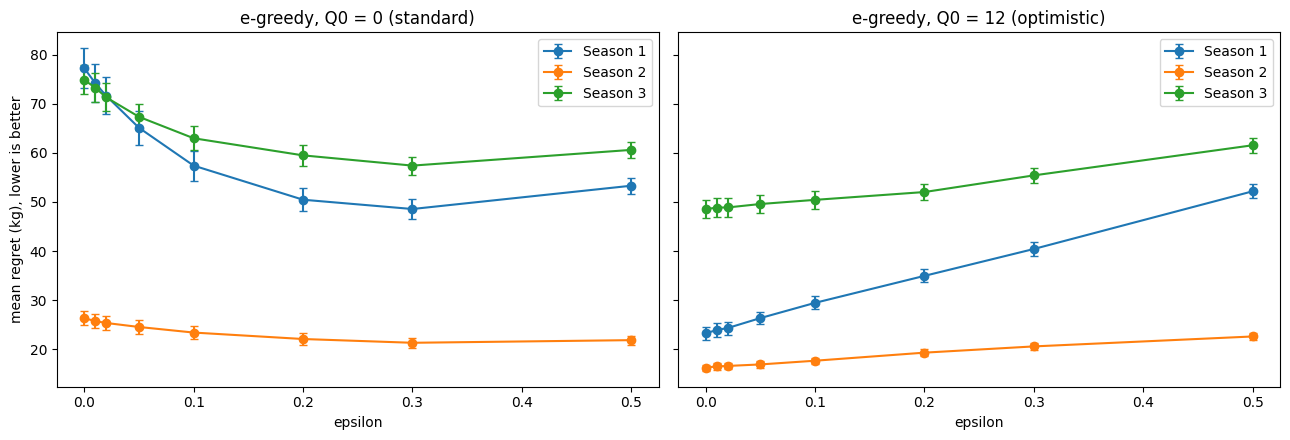
\includegraphics[width=\textwidth]{figures/task5_epsilon_sweep.png}
\caption{Decision regret distributions for the nine agents over 1,000 matched bays in each season.}
\label{fig:task5-regret}
\end{figure}


\subsection*{Comparison on the team's bays}
Through the notebook, we rebuilt each member's three bays and ran every agent with 200 seeds per bay. Table~\ref{tab:team-comparison} gives mean outcome regret over nine member-seasons and counts cases where an agent's mean catch exceeded the human result. Human regret averaged 47.6 kg; UCB and optimistic Greedy beat humans in seven cases each.

\begin{table}[H]\centering\small
\begin{tabular}{lrr}\toprule
Agent & Mean regret (kg) & Better than human (/9)\\\midrule
Human rule & 25.8 & 6\\
Random & 59.0 & 0\\
Greedy ($Q_0=0$) & 60.5 & 0\\
Greedy ($Q_0=12$) & 22.7 & 7\\
$\epsilon$-greedy ($Q_0=0$) & 45.7 & 4\\
$\epsilon$-greedy ($Q_0=12$) & 25.6 & 7\\
$\epsilon$-greedy ($\epsilon=0.1,\alpha=0.2$) & 53.9 & 3\\
UCB ($c=2$) & 22.2 & 7\\
UCB ($c=2,\alpha=0.2$) & 22.0 & 7\\\bottomrule
\end{tabular}
\caption{Average across nine logged team bays; agent outcome averages use 200 seeds per bay.}
\label{tab:team-comparison}
\end{table}

\subsection*{Best agents for Seasons 2 and 3}
Optimistic Greedy has the highest Season 2 mean (70.56 kg), but is practically tied with constant-step UCB (70.54 kg; ). UCB ($c=2$) leads Season 3 at 217.19 kg, with a modest $3.24\pm1.75$ kg advantage over HumanRuleAgent.

In a separate 200-day changing season, constant-step UCB reduced regret to 147.2 kg versus 167.1 kg for sample-average UCB.

\subsection*{Parameter study: epsilon-greedy}
We swept $\epsilon=0$--$0.5$ in each season with $Q_0=0$ and $Q_0=12$; Table~\ref{tab:epsilon-sweep} reports all tested regrets. The best tested value was $0.3$ for $Q_0=0$ and $0$ for $Q_0=12$. Optimistic values already explore, so random choices mainly reduce exploitation. 

\begin{table}[H]\centering\scriptsize
\begin{tabular}{rrrrrrr}\toprule
$\epsilon$ & S1 $Q_0=0$ & S2 $Q_0=0$ & S3 $Q_0=0$ & S1 $Q_0=12$ & S2 $Q_0=12$ & S3 $Q_0=12$\\\midrule
0.00 & 77.22 & 26.35 & 74.84 & 23.26 & 16.29 & 48.52\\
0.01 & 74.20 & 25.75 & 73.26 & 23.94 & 16.52 & 48.85\\
0.02 & 71.61 & 25.37 & 71.29 & 24.33 & 16.62 & 48.88\\
0.05 & 65.10 & 24.55 & 67.33 & 26.36 & 16.93 & 49.58\\
0.10 & 57.39 & 23.42 & 62.96 & 29.46 & 17.68 & 50.42\\
0.20 & 50.45 & 22.10 & 59.48 & 34.96 & 19.33 & 52.02\\
0.30 & 48.56 & 21.33 & 57.39 & 40.43 & 20.60 & 55.40\\
0.50 & 53.30 & 21.87 & 60.59 & 52.17 & 22.62 & 61.53\\\bottomrule
\end{tabular}
\caption{Mean regret (kg) over 1,000 matched bays for the epsilon sweep.}
\label{tab:epsilon-sweep}
\end{table}



Figure~\ref{fig:epsilon-sweep} shows the same parameter study graphically: exploration helps when $Q_0=0$, while optimistic initialization makes additional random exploration costly.


\begin{figure}[H]\centering
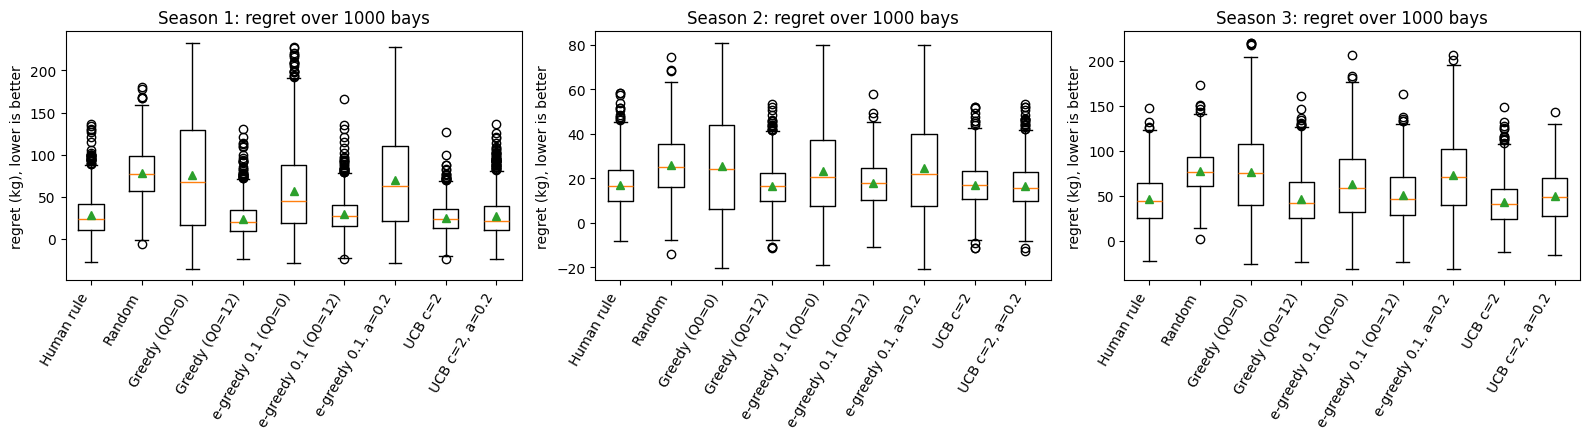
\includegraphics[width=0.92\textwidth]{figures/task5_regret_distributions.png}
\caption{Mean regret as $\epsilon$ varies, with standard and optimistic initial values.}
\label{fig:epsilon-sweep}
\end{figure}




\section*{Task 6: Contextual bandit}
\subsection*{Method and comparison}
For 300 days, the agent observes wind, waves and tide before each choice. Linear UCB fits a regularized catch model per spot from normalized conditions and adds an uncertainty bonus. We compared it with prediction-only selection, random selection and the best non-contextual policy on the same 1,000 bays.

\begin{table}[H]\centering\scriptsize
\begin{tabular}{lrrrrrr}\toprule
Agent & Mean & SD & Median & P10 & P90 & Regret\\\midrule
Random contextual & 1747.9 & 414.8 & 1743.1 & 1219.8 & 2290.1 & 1215.2\\
Prediction only ($\alpha=0$) & 1940.2 & 799.7 & 1871.8 & 951.4 & 3057.4 & 1022.9\\
Linear UCB ($\alpha=8$) & 2856.6 & 594.6 & 2854.9 & 2117.8 & 3600.3 & 106.5\\
UCB ($c=2$, ignores context) & 2790.2 & 651.9 & 2781.0 & 1965.4 & 3635.7 & 172.9\\\bottomrule
\end{tabular}
\caption{Contextual-bay total-catch distribution (kg) and mean oracle regret over 1,000 matched bays.}
\label{tab:context-results}
\end{table}

Linear UCB achieved the lowest regret (106.5 kg), beating non-contextual UCB (172.9 kg) and random on every bay. It averaged 2,856.6 kg; prediction-only averaged 1,940.2 kg (SD 799.7 kg). Without an uncertainty bonus, early noisy estimates can lead to poor exploitation: on seed 660, prediction-only caught 481.6 kg against an oracle of 4,203.3 kg, while Linear UCB caught 4,149.3 kg. Figure~\ref{fig:context-comparison} shows catches and paired gains over random.
\begin{figure}[H]\centering
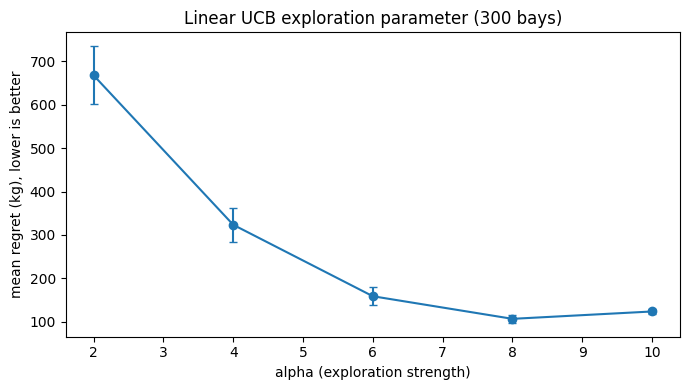
\includegraphics[width=0.92\textwidth]{figures/task6_alpha_sweep.png}
\caption{Contextual-agent catches and paired Linear UCB versus random comparison.}
\label{fig:context-comparison}
\end{figure}

\subsection*{Exploration parameter}
On 300 matched bays, regret fell from 667.5 kg at $\alpha=2$ to 107.0 kg at $\alpha=8$, then rose to 123.9 kg at $\alpha=10$. Moderate exploration helped learn condition-catch relationships; stronger exploration did not. Thus $\alpha=8$ was best in this sweep, not necessarily globally.
\begin{table}[H]\centering\small
\begin{tabular}{rrr}\toprule
$\alpha$ & Mean regret (kg) & SD regret (kg)\\\midrule
2 & 667.5 & 592.9\\
4 & 323.5 & 341.0\\
6 & 159.0 & 179.0\\
8 & 107.0 & 82.4\\
10 & 123.9 & 56.7\\\bottomrule
\end{tabular}
\caption{Linear UCB sensitivity to exploration strength over 300 matched contextual bays.}
\label{tab:context-alpha}
\end{table}


\begin{figure}[H]\centering
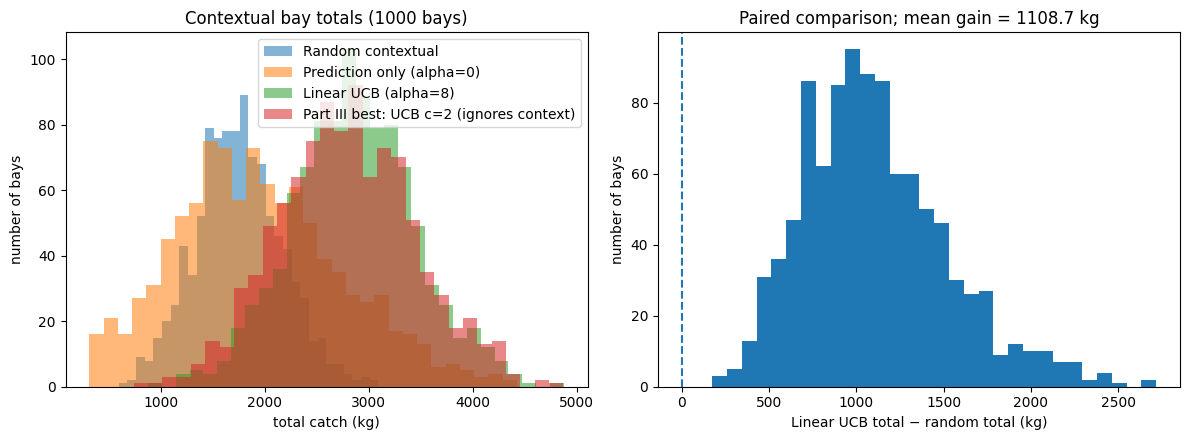
\includegraphics[width=0.70\textwidth]{figures/task6_contextual_comparison.png}
\caption{Mean regret and 95\% confidence intervals for the contextual $\alpha$ sweep.}
\label{fig:context-alpha}
\end{figure}




\newpage



\section*{Conclusion}
The experiments show that bandits need early exploration to identify productive spots, followed by exploitation. Optimistic Greedy and UCB performed strongly in stable seasons; UCB adapted best after the Season 3 shift. Expected-catch regret separated decision quality from random outcomes. Linear UCB also improved performance by using daily conditions. Exploration should therefore reflect both season dynamics and available information.




\section*{Team contributions}
Pu Meng, Dakio Isaac and Shane Elton Lewis each played all three seasons, supplied their own game logs and documented their strategies and results. 
\newline Pu Menggu designed the human rule agent and the masured the performance against the agents designed 
\newline Shane Elton Lewis designed the performance measure, greedy , epsilon greedy and UCB agent and analysed and specified all the agents used in the report 
\newline Dakio Isaac tested the designed performance measure in the simulator and separated decision from luckdesigned the contextual bandits agent using linear UCB and the UCB agent used in the project and specified it in the report 
\section{AI Use And Contribution}
This project used generative AI tools i.e. Claude AI , Gemini and Chatgpt to generate and debug the code used to simulate the N armed Bandit problem. 
\begin{thebibliography}{9}

\bibitem{sutton2018}
Sutton, R. S., \& Barto, A. G. (2018).
\textit{Reinforcement Learning: An Introduction}
(2nd ed.). The MIT Press.

\bibitem{claude}
\url{https://claude.ai/chat/7dc733a8-ac8a-46de-a1ee-3aa295d3d3d4}


\bibitem{claude2}
\url{https://claude.ai/chat/22a1aa81-9005-48a6-af82-20347d2c73ad}
\end{thebibliography}


\end{document}
